\documentclass[12pt, a4paper]{article}
\usepackage{graphicx} % Required for inserting images
\usepackage[final]{pdfpages}
\usepackage[serbian]{babel} % Use the Serbian language package
\usepackage{fontspec} % Required for using system fonts
\usepackage{geometry} % Required for setting page size
\usepackage{fancyhdr} % Required for custom headers and footers
\usepackage[scaled]{helvet}
\usepackage{csquotes}
\usepackage[colorlinks=true,linkcolor=black,citecolor=black,urlcolor=black]{hyperref} % Customize link colors
\usepackage[fixlanguage]{babelbib}
    \bibliographystyle{babunsrt}


% \setmainfont{Nimbus Sans L}
\setmainfont{Roboto}

\setlength{\parindent}{0pt}
\setlength{\parskip}{12pt}%

\geometry{a4paper, margin=1in}

% Customize headers and footers
\pagestyle{fancy}
\fancyhf{} % Clear header and footer
\fancyfoot[R]{\thepage} % Right align page number in the footer
\renewcommand{\headrule}{} % Remove header line


\begin{document}

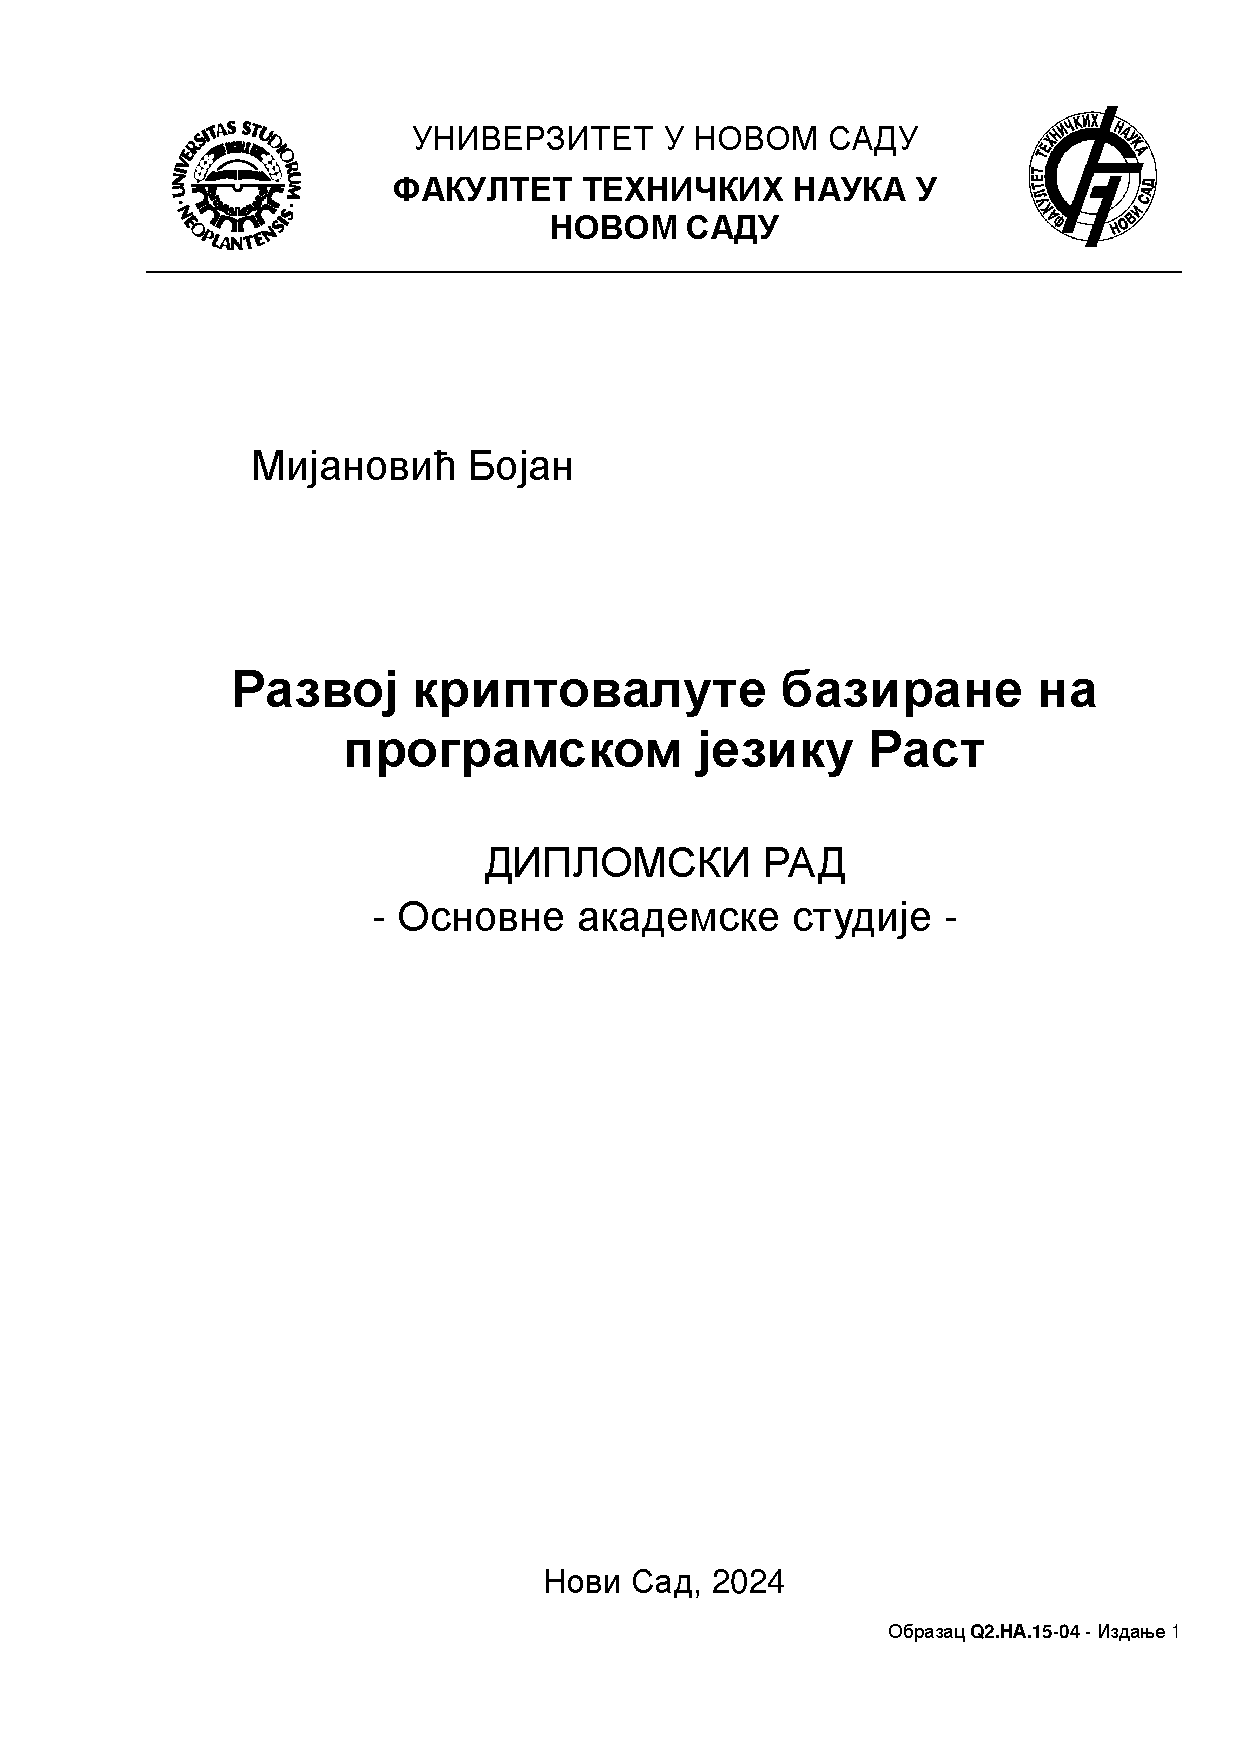
\includepdf[pages=-]{prva_strana.pdf}

\renewcommand{\contentsname}{Садржај}
\tableofcontents
\pagebreak

\section{Увод}
\textit{Blockchain} технологија представља дистрибутивну, децентрализовану и јавну базу свих трансакција \cite{1}.


Први концепт \textit{blockchain} технологије помиње се у 1982. години, када је Давид Чаум у својој дисертацији описао дистрибуирану базу података која користи криптографију \cite{2}. Овај рани рад није био директно повезан са дигиталним валутама, али је поставио темеље за будући развој \textit{blockchain} - а.

Права револуција долази 2008. године када Сатоши Накамото објављује рад "\textit{Bitcoin}: \textit{Peer-to-peer} електронски готовински систем", уводећи први модерни \textit{blockchain} и криптовалуту \textit{Bitcoin}. Генесис блок, први блок \textit{Bitcoin blockchain} - а, ископан је 3. јануара 2009. године, означавајући почетак \textit{blockchain} технологије какву данас познајемо \cite{3}.

\textit{Etherium}, лансиран 2015. године од стране Виталика Бутерина, увео је паметне уговоре који омогућавају сложеније трансакције и аутоматизацију различитих процеса. Овај развој проширио је примену \textit{blockchain} технологије далеко изван дигиталних валута, омогућавајући креирање децентрализованих апликација.

\textit{Blockchain} технологије су се од свог настанка имплементирале у различитим програмским језицима и окружењима. У својим раним фазама, \textit{blockchain} технологије су се углавном развијале користећи језике као што су \textit{C++} и \textit{Java}, захваљујући њиховој ефикасности и широкој употреби у индустрији. Касније, с појавом паметних уговора, \textit{Solidity} је постао стандард за развој на \textit{Etherium} платформи.

Овај рад се фокусира на имплементацију основних концепата \textit{blockchain} технологије у програмском језику \textit{Rust}, који је познат по својој сигурности, перформансама и могућности превенције грешака при руковању меморијом.

Рад је структуиран X целина
\pagebreak

\section{Основе \textit{Rust} програмског језика}
\textit{Rust} је савремени програмски језик који је развијен да буде безбедан и брз. Развијен од стране \textit{Mozilla Research}-а, \textit{Rust} је од свог настанка привукао велику пажњу због својих изузетних безбедносних карактеристика и перформанси.

\subsection{Увод у \textit{Rust} програмски језик}
\textit{Rust} је системски програмски језик који наглашава безбедност и брзину. За разлику од неких других језика, \textit{Rust} осигурава безбедност у раду са меморијом кроз свој јединствени систем власништва над подацима. То значи да \textit{Rust} омогућава програмерима да пишу брз и ефикасан код без страха од уобичајених грешака као што су сегментација или тзв. \textit{„dangling pointers“}. Поред тога, \textit{Rust} нуди снажне алате за паралелно програмирање, што га чини идеалним за развој сложених и ресурсоинтензивних апликација.

Због своје компајлиране природе и минималног \textit{runtime}-а, \textit{Rust} програми се извршавају ближе нивоу машинског језика, што резултује високим перформансама. Ово је кључно за \textit{blockchain} апликације где брзина обраде трансакција директно утиче на корисничко искуство и сигурност мреже.

\subsection{Зашто \textit{Rust} за \textit{blockchain}?}
Када је у питању развој blockchain апликација, \textit{Rust} се истиче као одличан избор из неколико разлога:
\begin{enumerate}
    \item \textbf{Безбедност меморије}: \textit{Rust}-ов систем власништва и провера за време компилације осигуравају да програмери избегну уобичајене грешке у раду са меморијом, што је критично за сигурност \textit{blockchain} система.
    \item \textbf{Перформансе}: \textit{Rust} је дизајниран да буде брз и ефикасан. Његов минималан \textit{overhead} и високо оптимизован компајлер резултирају брзим извршавањем кода, што је важно за обраду великог броја трансакција у реалном времену.
    \item \textbf{Паралелизам и конкурентност}: \textit{Rust} нуди снажну подршку за паралелно и конкурентно програмирање, омогућавајући оптимално коришћење мулти-језгарних процесора.
\end{enumerate}

\textit{Rust} нуди низ алата и библиотека које олакшавају развој сложених апликација. Две од најзначајнијих библиотека за развој \textit{blockchain} апликација су \textit{Tokio} и \textit{libp2p}. Ове библиотеке пружају подршку за асинхроне позиве и \textit{peer-to-peer} комуникацију, што је кључно за функционалност и ефикасност \textit{blockchain} система.

\textbf{\textit{Tokio}} је моћна асинхрона \textit{runtime} библиотека за \textit{Rust} која омогућава развој високоперформансних и високо доступних апликација. Кроз \textit{Tokio}, програмери могу да имплементирају асинхроне позиве и да развију веб сервере који могу да обрађују велики број истовремених веза.

\textit{\textbf{libp2p}} је модуларни мрежни стек који омогућава \textit{peer-to-peer} комуникацију. У контексту \textit{blockchain}-а, \textit{libp2p} се користи за омогућавање комуникације између различитих чворова у мрежи. Ова библиотека је флексибилна и подржава различите протоколе за пренос података, што је чини идеалном за развој децентрализованих апликација.

\pagebreak

\section{Увод у \textit{blockchain} технологију}
\textit{Blockchain} технологија представља савремен приступ складиштењу и дистрибуцији података. Основни принципи и концепти \textit{blockchain} технологије нуде дубоку промену у начину на који се информације похрањују, проверавају и дистрибуирају путем децентрализоване мреже рачунара.

\subsection{Основни принципи и концепти}
\textit{Blockchain} се може дефинисати као дистрибуисана дигитална књига трансакција. Основна идеја је стварање низа блокова који садрже податке. Блкови су криптографски повезани тако да је немогуће мењати податке у претходним блоковима без мењања свих следећих блокова. 

Кључни елементи блокчејна укључују:
\begin{enumerate}
    \item \textbf{Децентрализација}: Подаци се похрањују и управљају путем мреже чворова уместо централизованог ауторитета, што осигурава транспарентност и отпорност на цензуру.
    \item  \textbf{Дистрибуираност}: Сваки чвор у мрежи садржи комплетан или део \textit{blockchain}-а, омогућујући свима у мрежи да виде исте податке. Ово спречава појединачне тачке квара и повећава отпорност на нападе.
    \item \textbf{Сигурност}: Криптографски алгоритми осигуравају да је свака промена у \textit{blockchain}-у лако проверљива, а трансакције се потврђују кроз консензус мреже.
    \item \textbf{Неповратност}: Након што је трансакција забележена у \textit{blockchain}-у, тешко ју је променити или обрисати без сагласности већине чворова у мрежи, чиме се осигурава поверење и интегритет података.
\end{enumerate}


\subsection{Поређење са традиционалним базама података}
Насупрот традиционалним базама података које су често централизоване и ослањају се на поверење у једну јединицу, \textit{blockchain} нуди неколико кључних разлика:
\begin{enumerate}
    \item \textbf{Централизација у односу на децентрализацију}: Традиционалне базе података често су централизоване под контролом једне организације. \textit{Blockchain} дистрибуише податке широм мреже, елиминишући потребу за централним ауторитетом.
    \item \textbf{Транспарентност и проверљивост}: \textit{Blockchain} омогућава свим корисницима увид у све трансакције које су се догодиле, што повећава транспарентност и смањује могућност манипулације.
    \item \textbf{Сигурност и отпорност}: Због своје дистрибуиране природе, \textit{blockchain} је отпорнији на нападе и кварове у поређењу са традиционалним базама података које су осетљиве на појединачне тачке квара.
    \item \textbf{Ефикасност и трошкови}: Иако \textit{blockchain} може бити спорији у обради података у поређењу са централизованим базама података, његова сигурност и транспарентност могу надмашити трошкове и ризике традиционалних система.
\end{enumerate}










\pagebreak

\section{Литература}
\renewcommand{\refname}{}
\vspace{-\parskip} % Remove extra space added by \parskips
\vspace{-\parskip} % Remove extra space added by \parskips
\vspace{-\parskip} % Remove extra space added by \parskips
\vspace{-\parskip} % Remove extra space added by \parskips
\bibliography{bibliography}



\end{document}

